\documentclass[twocolumn]{article}

% Load packages
\usepackage[margin=1in]{geometry}
\usepackage{lipsum}
\usepackage{graphicx}
\usepackage{caption}
\usepackage{subcaption}
\usepackage{amsmath}
\usepackage{amsfonts}
\usepackage[backend=biber, style=numeric]{biblatex}

% Set font
\usepackage{cmbright}
\renewcommand{\familydefault}{\sfdefault}

% Set new carrier line at the end of each paragraph with double interline
\usepackage[parfill]{parskip}
\setlength{\parskip}{\baselineskip}

% Set title and abstract to span full width
\usepackage{titling}
\pretitle{\begin{center}\LARGE\bfseries}
\posttitle{\par\end{center}\vskip 0.5em}
\preauthor{\begin{center}
\large \lineskip 0.5em}
\postauthor{\end{center}}
\setlength{\droptitle}{-2cm}
\usepackage{abstract}
\renewcommand{\abstractname}{}    % clear the abstract title
\renewenvironment{abstract}
{\begin{center}\bfseries\abstractname\vspace{-0.5em}\end{center}\list{}{%
\setlength{\leftmargin}{0.5in}
\setlength{\rightmargin}{\leftmargin}%
}%
\item\relax}
{\endlist}

% Set bibliography
\addbibresource{references.bib}

% Set author section with pictures
\usepackage{authblk}
\renewcommand\Authands{ and }
\setlength{\affilsep}{0.5cm}

% Set document title and authors
\title{Document Title}
\author[1]{Author One\thanks{Corresponding author: author.one@email.com}}
\author[2]{Author Two}
\author[3]{Author Three}
\affil[1]{Department of X, University of Y}
\affil[2]{Department of A, University of B}
\affil[3]{Department of C, University of D}
\date{}

% Set caption format
\DeclareCaptionLabelFormat{myformat}{Fig. #2}
\captionsetup{labelformat=myformat}

\begin{document}

% Print title
\maketitle

% Print abstract
\begin{abstract}
\lipsum[1-3]
\end{abstract}

% Start two-column layout
\begin{twocolumn}

% Introduction section
\section{Introduction}
\lipsum[4-10]

% Example equation
\begin{equation}
    f(x) = x^2 + 2x + 1
\end{equation}

% Example figure
\begin{figure}[htbp]
    \centering
    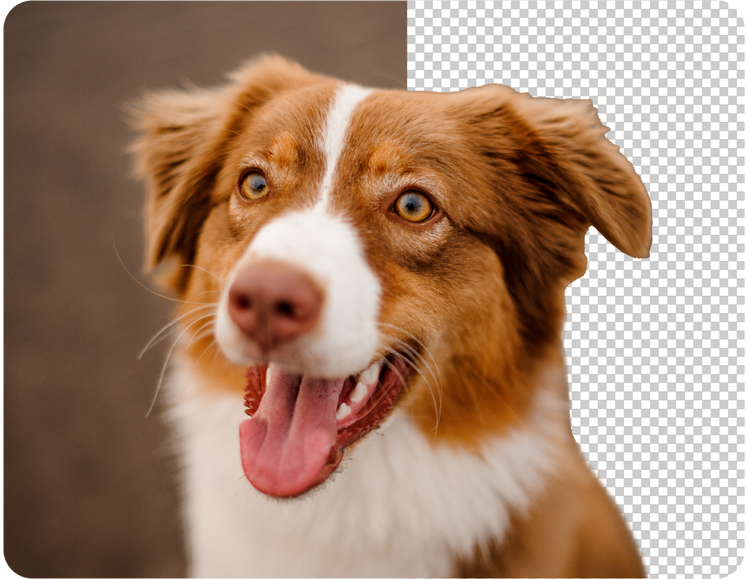
\includegraphics[width=0.8\columnwidth]{example_figure.png}
    \caption{Example figure caption.}
    \label{fig:example}
\end{figure}

% Text with citation
According to \cite{example-article}, this is an example citation. Another example is given in \cite{example-book}.

According to \cite{example-article}, this is an example citation. Another example is given in \cite{example-book}.

% Example table
\begin{table}[htbp]
    \centering
    \caption{Example table caption.}
    \label{tab:example}
    \begin{tabular}{c|c}
        Column 1 & Column 2 \\
        \hline
        1 & 2 \\
        3 & 4 \\
    \end{tabular}
\end{table}

% Conclusion section
\section{Conclusion}
\lipsum[5-6]

% Print bibliography
\printbibliography

% End two-column layout
\end{twocolumn}

% Author section with pictures
% Set author information
\newcommand{\authorName}{John Doe}
\newcommand{\authorAffiliation}{Department of Example, Institution}
\newcommand{\authorBio}{
    \lipsum[1] % Replace with author bio
}

% Author picture
\begin{figure}[htbp]
    \centering
    \includegraphics[width=0.3\textwidth]{example-image} % Replace with author picture
    \caption{\authorName}
\end{figure}

% Author information
\section*{\authorName}
\begin{itemize}
    \item \textbf{Affiliation:} \authorAffiliation
    \item \textbf{Email:} john.doe@example.com
\end{itemize}

% Author biography
\section*{Biography}
\authorBio

\end{document}